\documentclass{article}
\usepackage{float}

% Language setting
% Replace `english' with e.g. `spanish' to change the document language
\usepackage[english]{babel}

% Set page size and margins
% Replace `letterpaper' with`a4paper' for UK/EU standard size
\usepackage[letterpaper, top=1.5cm, bottom = 1.5cm, left = 1.5cm, right = 1.5cm, marginparwidth=1.75cm]{geometry}

% Useful packages
\usepackage{amsmath}
\usepackage{graphicx}
\usepackage[colorlinks=true, allcolors=blue]{hyperref}

\title{Exploring the relationship between climate attitudes and extreme weather events - S\&DS 625 Final Project}
\author{Megan Ayers}


\begin{document}
\maketitle

\section{Introduction}
\subsection{Contextualizing and motivating}
Climate change and environmental degradation is one of the most existential
crises of our time, if not the most existential. Unfortunately, many
Americans do not agree with this statement and/or do not fully comprehend the
implications of our global future if we do not address the causes of
climate change. Without recognition of the seriousness of climate change,
harmful consumer habits perpetuate, eco-friendly policies falter due to lack
of support, and the industries and corporations that negatively impact the
environment are not held accountable nor pressured to abandon the status-quo.
Climate communication is a field that works with these issues, and in
particular, with how to educate and persuade individuals about climate
change and the necessity of acting to reduce it. The hope is that
the more people there are that recognize climate change as a serious threat,
the more likely we are to have politicians and corporations that are
pressured to use their positions of power to enact positive change when it
comes to the environment. 

This contextualizes the goal for this final project - to better understand
some aspects of climate change beliefs at the county-level. If we don't 
understand the beliefs that people currently have about climate change,
and what factors might influence those beliefs, then we will be less
effective at trying to persuade those people than if we can be understanding
and empathetic at the same time as being convincing. In particular, this
report investigates how local extreme weather events relate to county-level
climate change beliefs. Perhaps personally experiencing one of
the widely broadcasted affects of climate change - increased extreme weather
events such as drought, hurricanes, wildfires, winter storms, etc - would
cause a person to take climate change more seriously, compared to someone
who just hears about these things happening on the news. However, there are
other cultural and demographic factors that are expected to have an effect
on climate change opinions that also need to be controlled for, such as
political leanings and age.


\subsection{Data sources}
To explore the relationship between extreme weather events and climate
change opinion with consideration given to the additional impact of
political leanings and demographics on climate change beliefs, the analysis
draws on information from multiple data sources. 

Data collected and processed by the Yale Program on Climate Change
Communication is used to understand climate change belief (the response
variable of this analysis). This data consists of US
county-level estimates of climate change beliefs, i.e. x\% of the population
in New Haven County believes that climate change is happening. These
estimates are calculated from a large-scale nation-wide survey (n > 25,000)
conducted in spring of 2020, and were "derived from a statistical model using
multilevel regression with post-stratification (MRP)". Though using
individual-level data could be more convincing for arguing existence of a
relationship between extreme weather event experiences and climate change
beliefs (the unit "county" does not itself have a climate change belief),
actually obtaining the supplementary data at this level was not feasible for
this project due to data privacy issues. 

Supplementary demographic data at the county level was collected from the Census
Bureau's ACS 2019 estimates using the R package `tidycensus`. To understand
the political leaning of each county, 2020 general election results were obtained
at the county level. These came from a data set containing general election
results from 2000-2020 maintained by the MIT Election Data and Science Lab
and accessed via the Harvard Dataverse. 

Identifying counties that experienced an extreme weather event around the
time of the climate opinion survey is not cut-and-dried. How should one
define "extreme weather"? There may be multiple reasonable responses
to this question, but this report defines "extreme weather" as
weather events that were declared disasters by FEMA
(Federal Emergency Management Agency). Records of these events from 1953 to
2021 are recorded in the online OpenFEMA Data Sets at the state and county level.
FEMA disasters were chosen as the indicator of extreme weather because
they signal a disaster beyond what state governments typically expect and are
prepared to handle. This accounts for the fact that independently of climate
change, some parts of the country naturally experience - and are used to
experiencing - more severe weather than others.


\section{Data Preparation}

Merging these data sources required considerable cleaning and quality
assurance checks of each individual source.

\subsection{Climate change opinion survey data}
Because the providers of the climate change opinion survey already processed
the individual responses into county-level estimates, this data is very clean
to begin with. Data is available for every county reported on by the Census
in 2020, there are no duplicate rows, and the response variable `happening`
(indicating the proportion of county population that believes climate change
is happening) is relatively Normal in distribution. Note that the original
survey file contains data for many different climate-related questions asked
in the survey, but for this analysis I am just focusing on the high level
question of existence of climate change.

\subsection{Election data}
This data set required a little more work to clean up. Data was reported for
one county that was not recognized as a by the Census, and was dropped. For
some reason, San Joaquin County CA had missing data, which I was able to 
manually find from the county website and replace. Votes were sometimes
recorded by the mode in which they were received (ex. "Early Vote", 
"Absentee", "Election Day" etc.) and sometimes in total, so aggregation to 
the total county level had to be standardized between counties. I was able
to rectify all differences in county names between this source and the 
Census Bureau (which I regarded as ground truth for standardizing all sources
to use FIPS codes for future merging) except for voting districts in Alaska.
I was unable to find a way to map voting districts to Census-reported
counties, so I dropped Alaska from the analysis. Although the other data
sources do have information on Alaska, I found political leaning to be such a
strong indicator of climate change belief that I think it is preferable to
drop it entirely from the analysis rather than introduce missing values for
political leaning.
Figure 1 shows the geographic distribution of the county-level 2020 election
results, while also indicating whether that county has above or below average
belief in climate change (compared to the political group average, not the
overall average).

\subsection{Census demographic data}
The ACS 2019 estimates obtained through the Census were very clean and
required almost no cleaning aside from reshaping the data and renaming one
county to be consistent with a recent name change. I began the analysis with
information about the gender, race, and ethnicity breakdowns of each county,
along with the median income and age of each county. I calculated population
proportions to use in the analysis instead of the raw total counts.

\subsection{FEMA weather data}
Given the choice of the FEMA data set, there remains a tension between the
ideas that experiencing multiple events over a longer time scale would have
a larger impact on people's mindsets, but also that it is harder to safely
assume that the same individuals are remaining in the same county over a
longer time scale. In an attempt to balance these competing interests,
counties are flagged as "affected by extreme weather" if they experienced
a FEMA declared event in 2019 (the closest data to when the climate opinion
survey was collected), and also experienced at least 2 FEMA declared events
between 2015-2018. This second requirement is an attempt to capture counties
where extreme weather is more likely to be seen as recurrent rather than a
fluke. 511 (a little over 16\%) US counties meet this requirement. Note that
the original data sets include FEMA disasters that are non-weather related,
such as earthquakes, biological disasters, chemical disasters, terrorist
disasters, etc. This analysis considers hurricanes, floods, severe storms,
fires, snow, tornados, severe ice storms, coastal storms, typhoons, and
droughts. Figure 2 displays all FEMA declared weather disasters from 2015-2019,
as well as highlighting the counties which meet the requirements outlined above
to be considered as "affected by severe weather" in the analysis.

\begin{figure}[H]
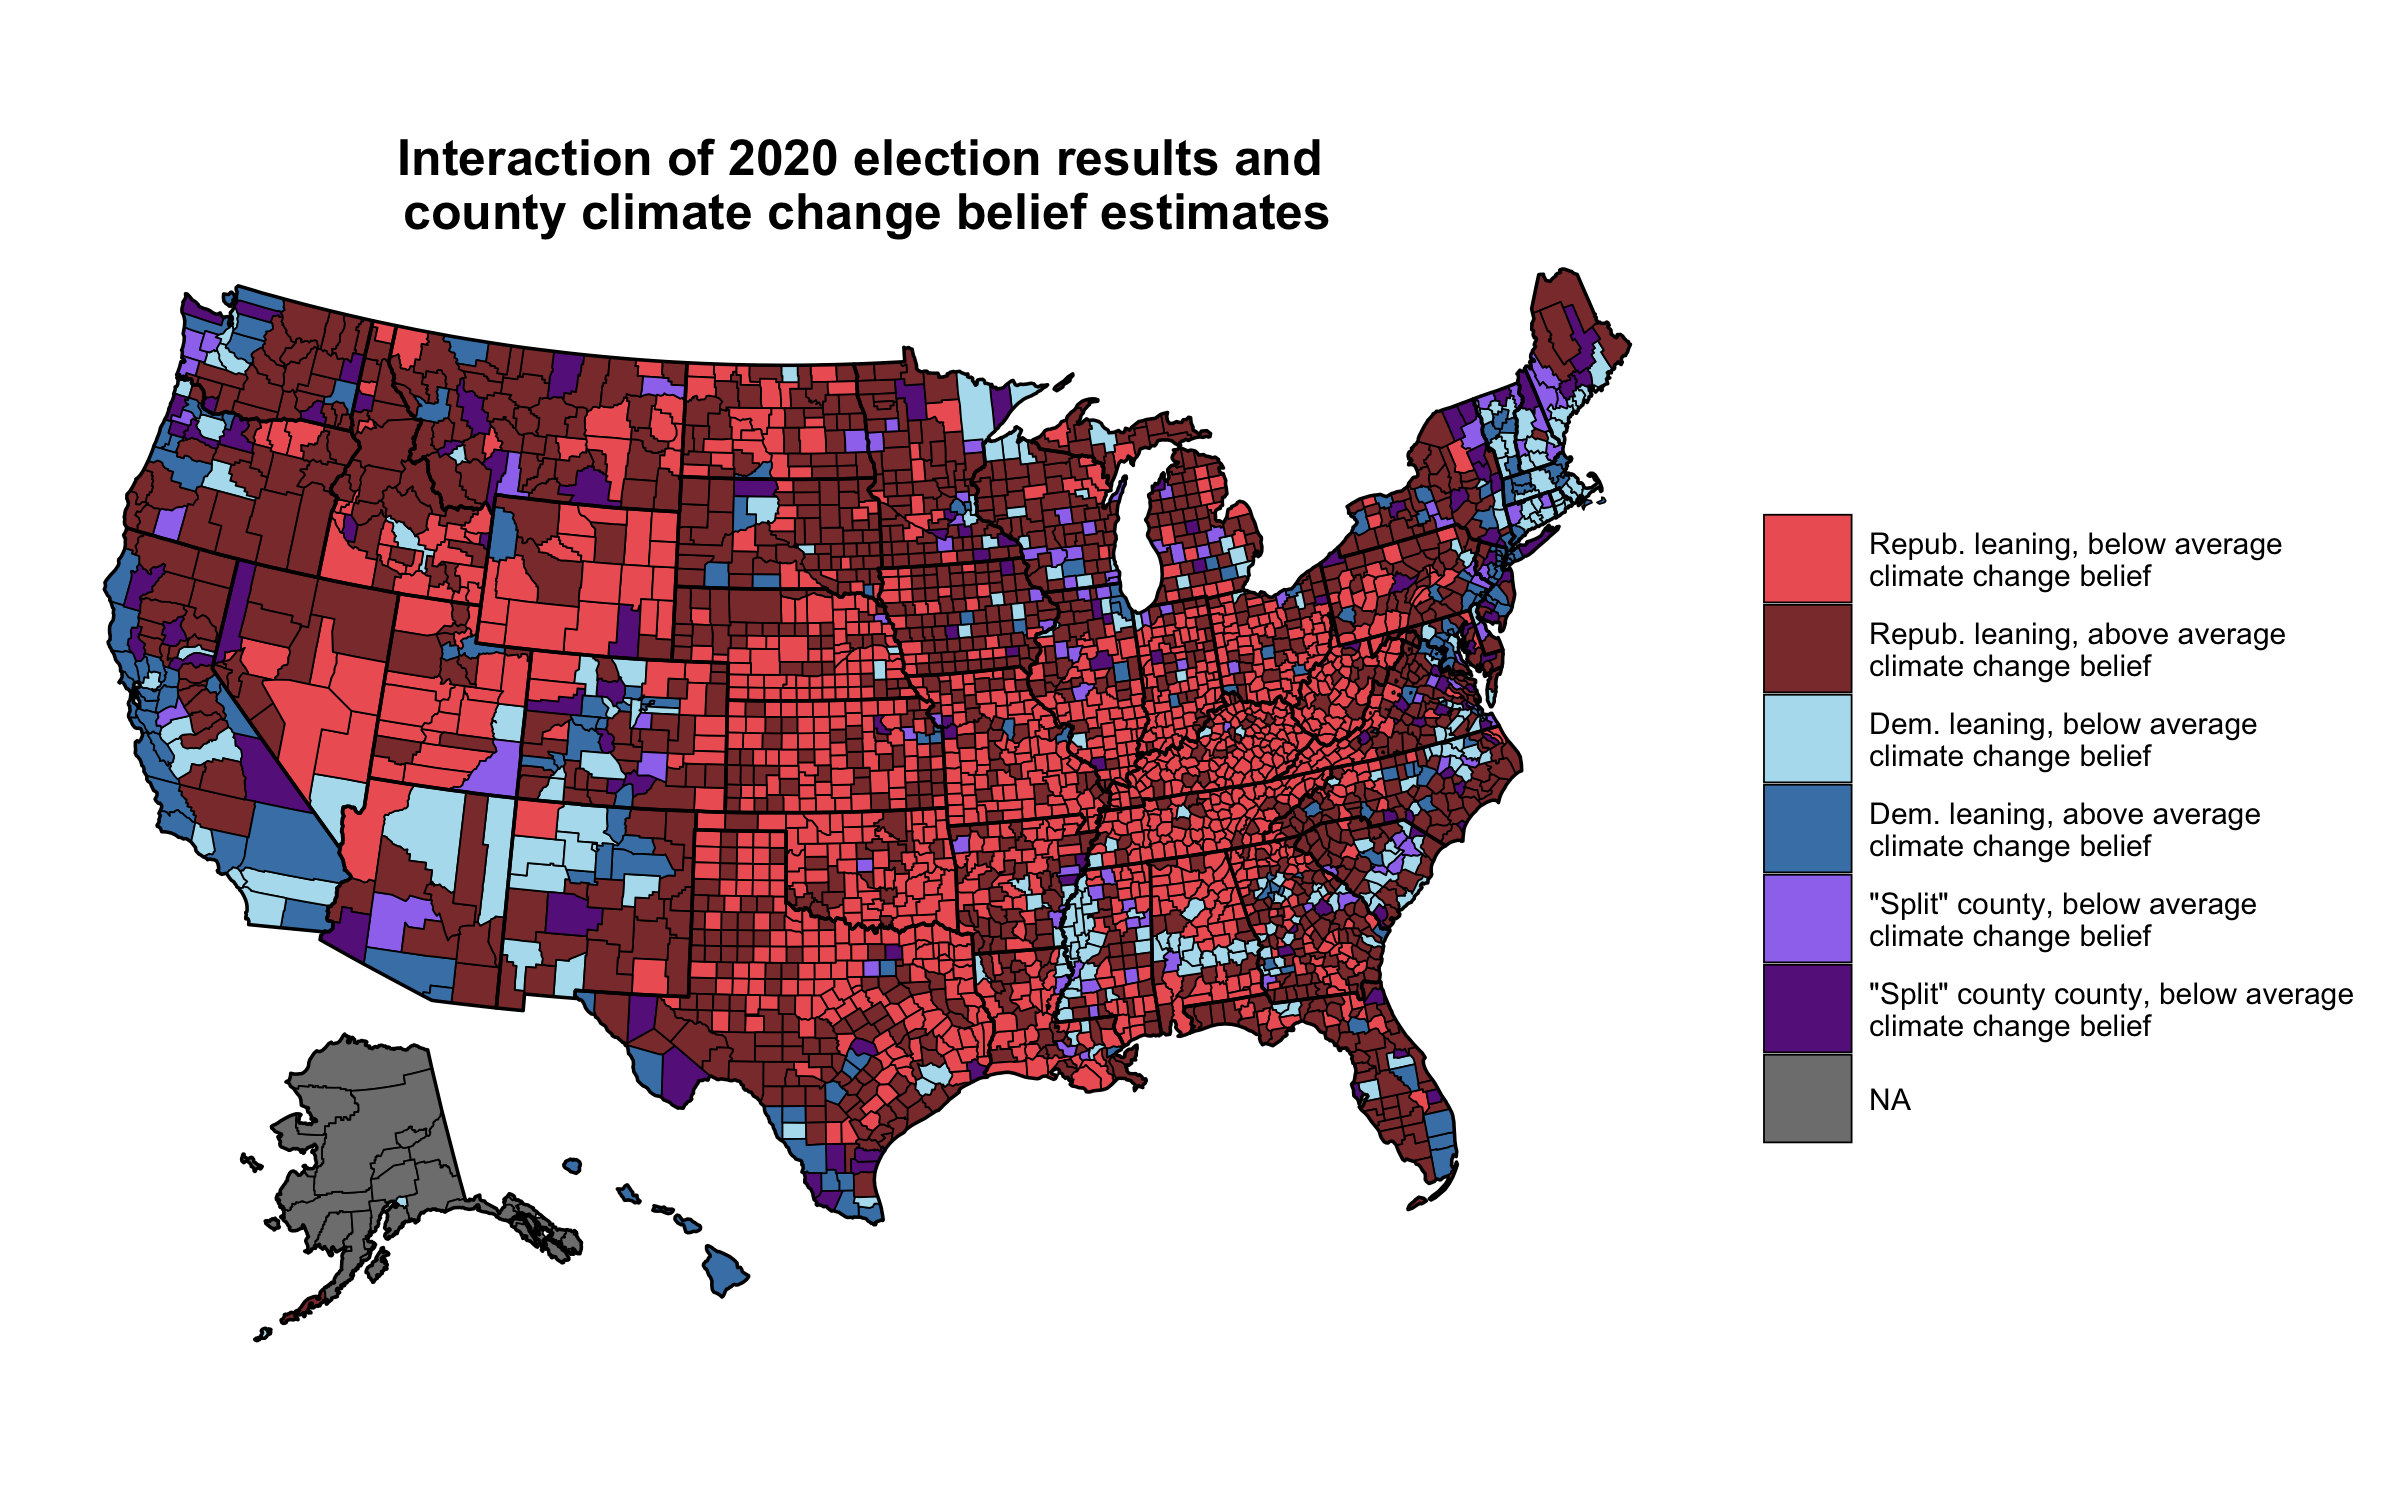
\includegraphics[scale=0.225]{images/election_climate_beliefs_map_in_group_comp.png}
\caption{This figure shows the 2020 presidential election results at the county level while also showing whether these counties have climate change belief above/below average compared to their political group. "Split" counties refers to counties where neither Democrats nor Republicans won more than 52.5\% of the vote.}
\end{figure}


\begin{figure}[H]
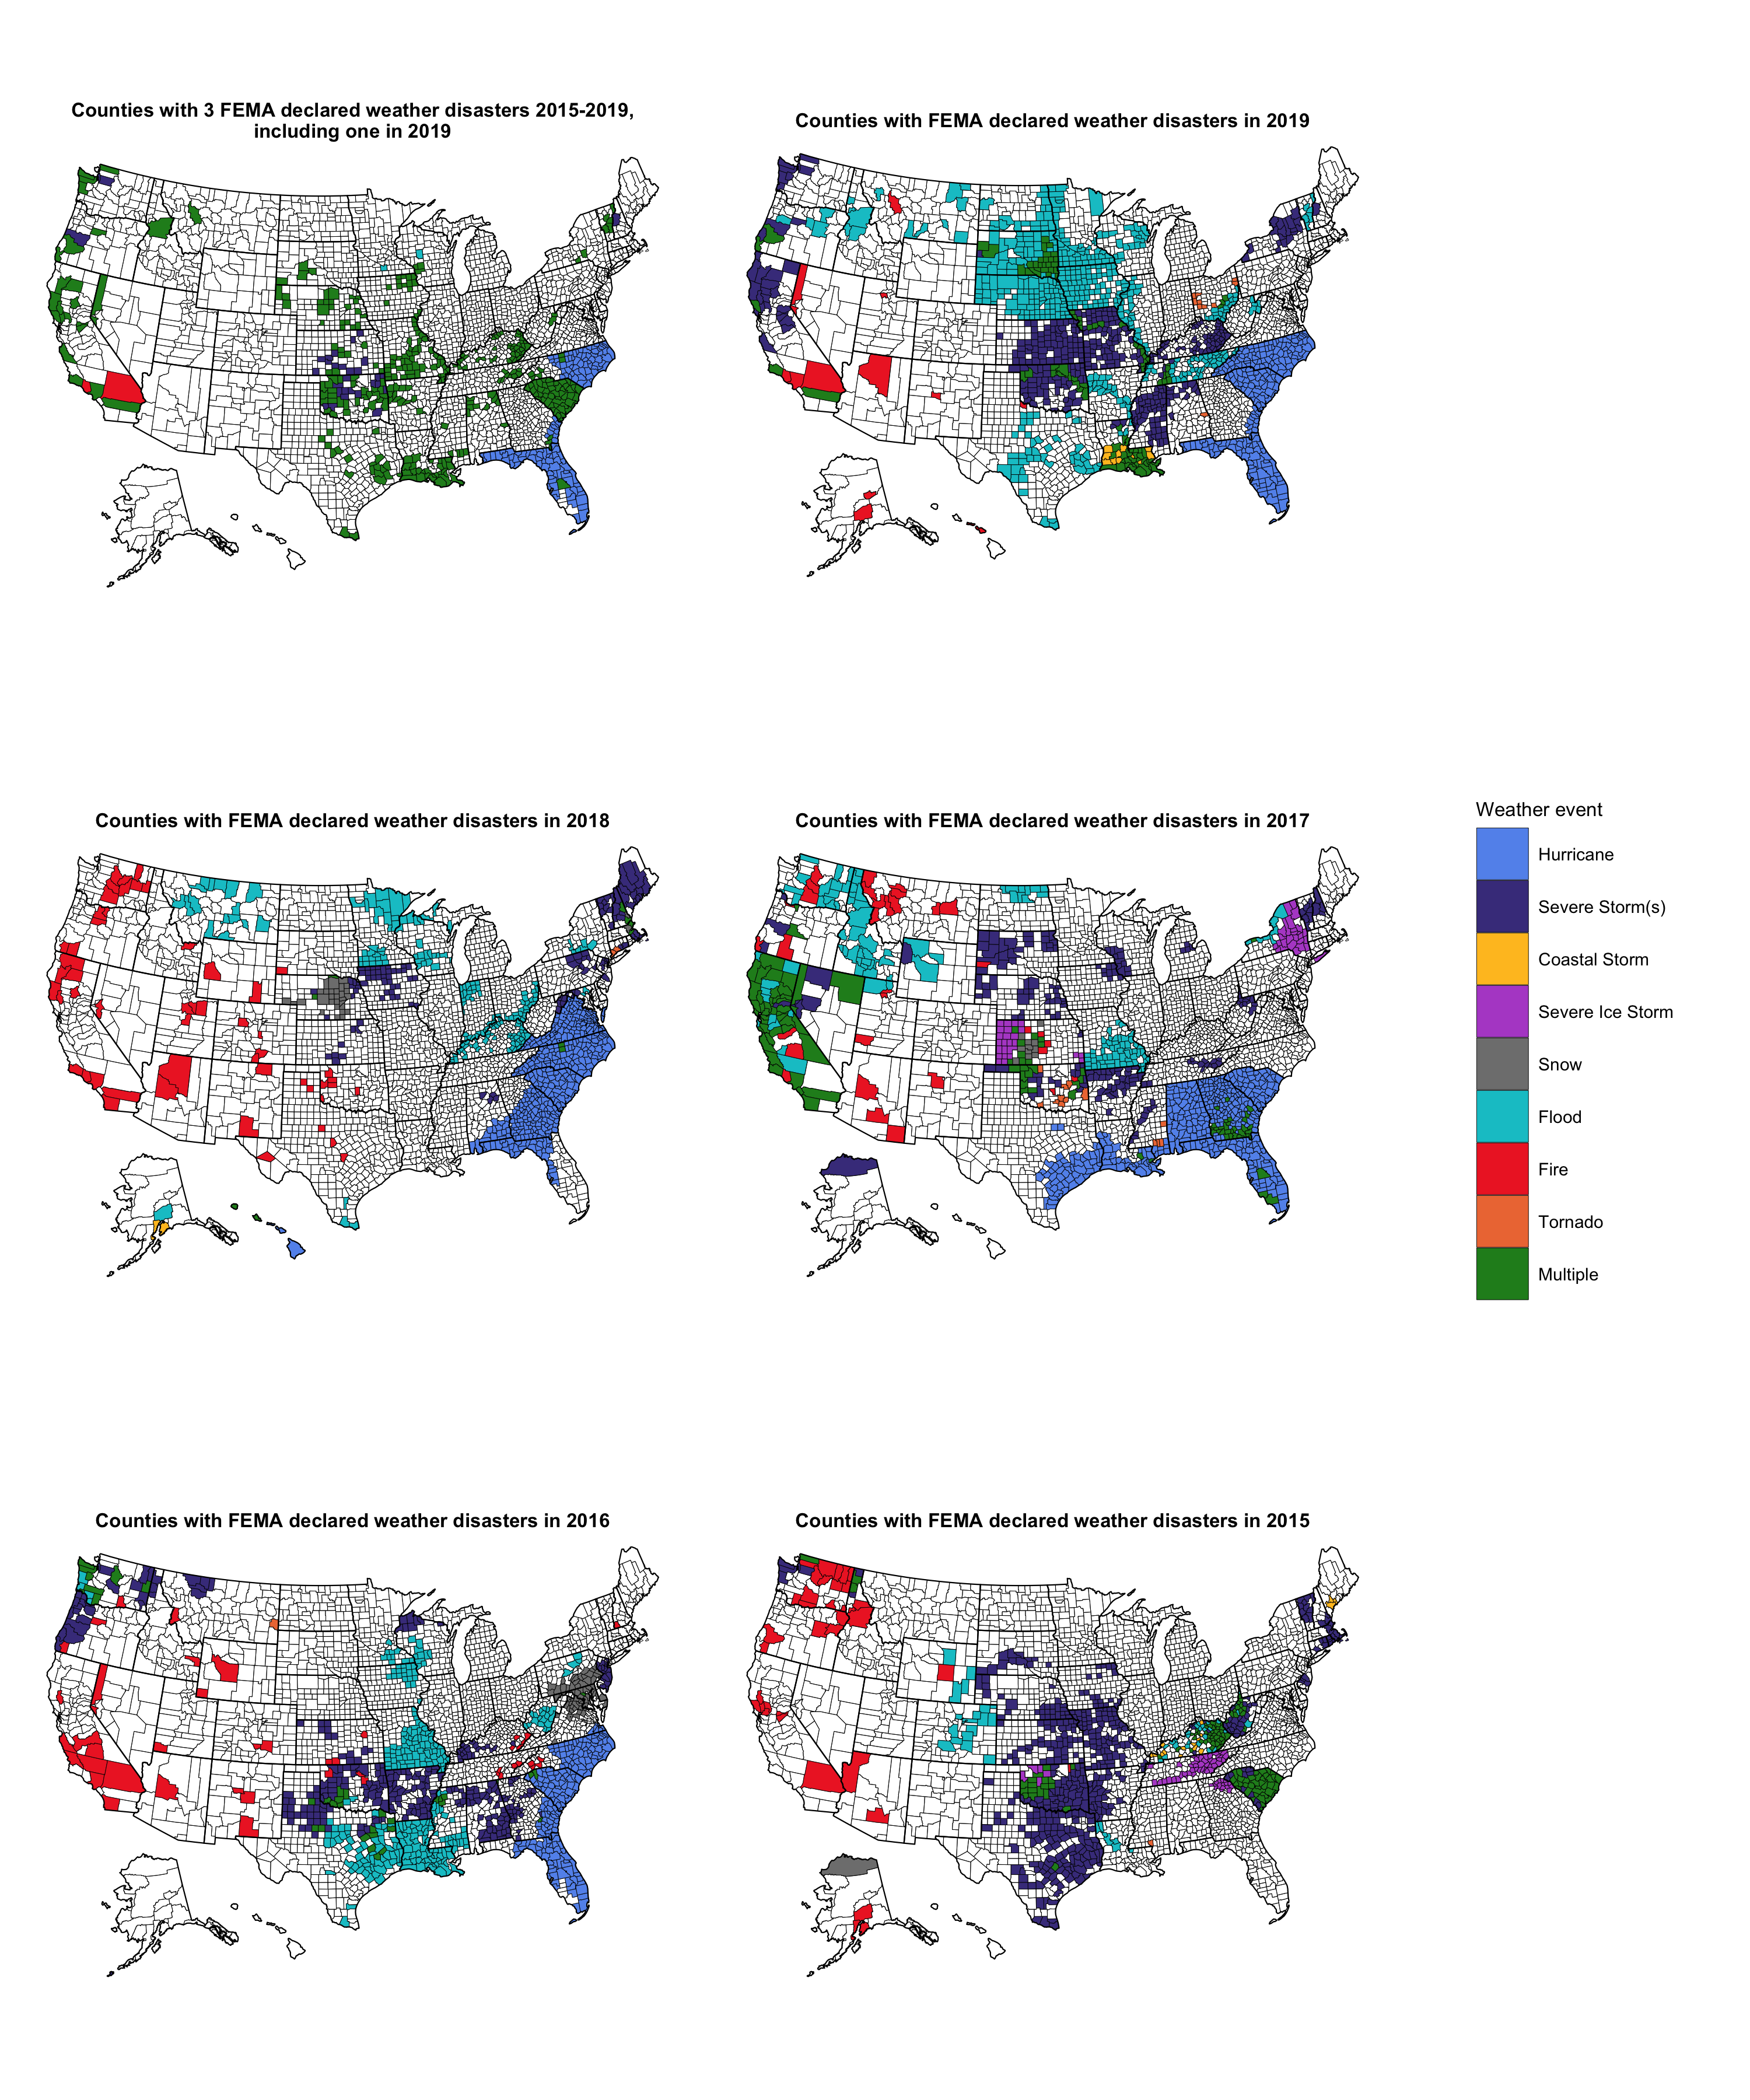
\includegraphics[scale=0.175]{images/fema_events_maps_combined.png}
\caption{Upper left: counties with FEMA declared disasters that are flagged as "affected by severe weather" in this analysis. The rest of the plots show all FEMA declared weather disasters from 2015-2019. Larger plots are available in code directory.}
\end{figure}



\section{Analysis}

\textcolor{red}{Remember to discuss ideas inspired by Causal Inference but
not actually valid in that framework}
Furthermore, it is difficult to guarantee that an
individual experienced an extreme weather event, even if they are recorded
as living in the county where one occurred, and "treatment" of experiencing
a weather event is not randomized.

\textcolor{red}{Try repeating analysis with just hurricanes}

\section{Results}
\section{Conclusion}
\section{References}

\subsection{Contextualizing the problem of climate change and climate change communication}
\begin{itemize}
	\item Guardian article about current climate change crisis: \url{https://www.theguardian.com/environment/ng-interactive/2021/oct/14/climate-change-happening-now-stats-graphs-maps-cop26}
	\item Organization for climate change communication: \url{https://climate-xchange.org/communicating-the-climate-crisis/}
\end{itemize}

\subsection{Data sources}
\begin{itemize}
	\item Yale Climate Communication Group: \url{https://climatecommunication.yale.edu/}
	\item Climate change opinion data: \url{https://climatecommunication.yale.edu/visualizations-data/ycom-us/}
	\item Election data: MIT Election Data and Science Lab, 2018, "County Presidential Election Returns 2000-2020", \url{https://doi.org/10.7910/DVN/VOQCHQ}, Harvard Dataverse, V9, UNF:6:qSwUYo7FKxI6vd/3Xev2Ng== [fileUNF]
\end{itemize}

\subsection{Analysis documentation}
\begin{itemize}
	\item MatchIt package: \url{https://kosukeimai.github.io/MatchIt/reference/method_optimal.html}
	\item TidyCensus package: \url{https://cran.r-project.org/web/packages/tidycensus/tidycensus.pdf}
\end{itemize}



\end{document}